% !TEX root = ./amsa_main.tex
\section{Numerical Experiments}\label{sec:numerical}
We illustrate the behavior of coordinate update algorithms for solving portfolio optimization, image processing, and machine learning problems. Our primary goal is to show the efficiency of coordinate update compared to the corresponding full update algorithms. We will also illustrate that asynchronous parallel coordinate update algorithms are more scalable than their synchronous parallel counterparts. 

Our first two experiments run on Mac OSX 10.9 with 2.4 GHz Intel Core i5 and 8 Gigabytes of RAM. The experiments were coded in Matlab. The sparse logistic regression experiment runs on 1 to 16 threads on a machine with two 2.5Ghz 10-core Intel Xeon E5-2670v2 (20 cores in total) and $64$ Gigabytes of RAM. The experiment was coded in C++ with OpenMP enabled. We use the Eigen library\footnote{\url{http://eigen.tuxfamily.org}} for sparse matrix operations.

\cut{\subsection{Least Square}\label{lsqexperiment2}
In this subsection, we compare the efficiency of four different coordinate update schemes (cyclic, cyclic shuffle, random, and greedy with Gauss-Southwell rule) with the full gradient descent method for solving the least square problem
$$\Min_{x} \frac{1}{2} \|A x - b\|^2,$$
where $A \in \RR^{m \times n}$ and $b \in \RR^m$. We solve the above problem with the following update scheme
$$x^{k+1} = x^k - \eta_k A^{\top}(A x^k - b),$$
where $\eta_k$ is the step size. This test uses three datasets, which are summarized in Table \ref{tab:ls-data}.  
\begin{table}[!hbtp]
\centering
 \begin{tabular}{lrrrr}
  \toprule
     & $m$  & $n$ & $A$ & $b$\\
   \midrule
   Dataset I & 1000 & 1000 & \texttt{diag([1:m])} & \texttt{ones(m, 1)} \\
   Dataset II & 1000 & 500 & \texttt{randn(m, n)} & \texttt{ones(m, 1)} \\
   Dataset III & 1000 & 500 & \texttt{rand(m, n)} & \texttt{ones(m, 1)} \\
   \bottomrule
\end{tabular}
 \caption{Three datasets for the least square problem\label{tab:ls-data}}
\end{table}

For both full gradient descent method and greedy coordinate update method with Gauss-Southwell rule, the step size $\eta$ is set to $\frac{2}{\|A\|_2^2}$. For the other three methods, if coordinate $i$ is selected, then $\eta_k$ is set to $\frac{1}{(A^{\top}A)_{ii}}$. Figure \ref{fig:ls_a} shows that for Dataset I, both cyclic update and cyclic shuffle update converge to the optimal solution with one epoch. Random coordinate update converges to the optimal solution after $8$ epochs. However, the gradient descent algorithm and greedy algorithm converge very slowly. This is due to the small step size ($\eta_k = 10^{-6}$). For the other two datasets, we observe that random coordinate update and cyclic shuffle coordinate update give consistent better performance than the full gradient descent algorithm. 
\begin{figure}[!htbp] \centering
    \begin{subfigure}[b]{0.3\linewidth}
        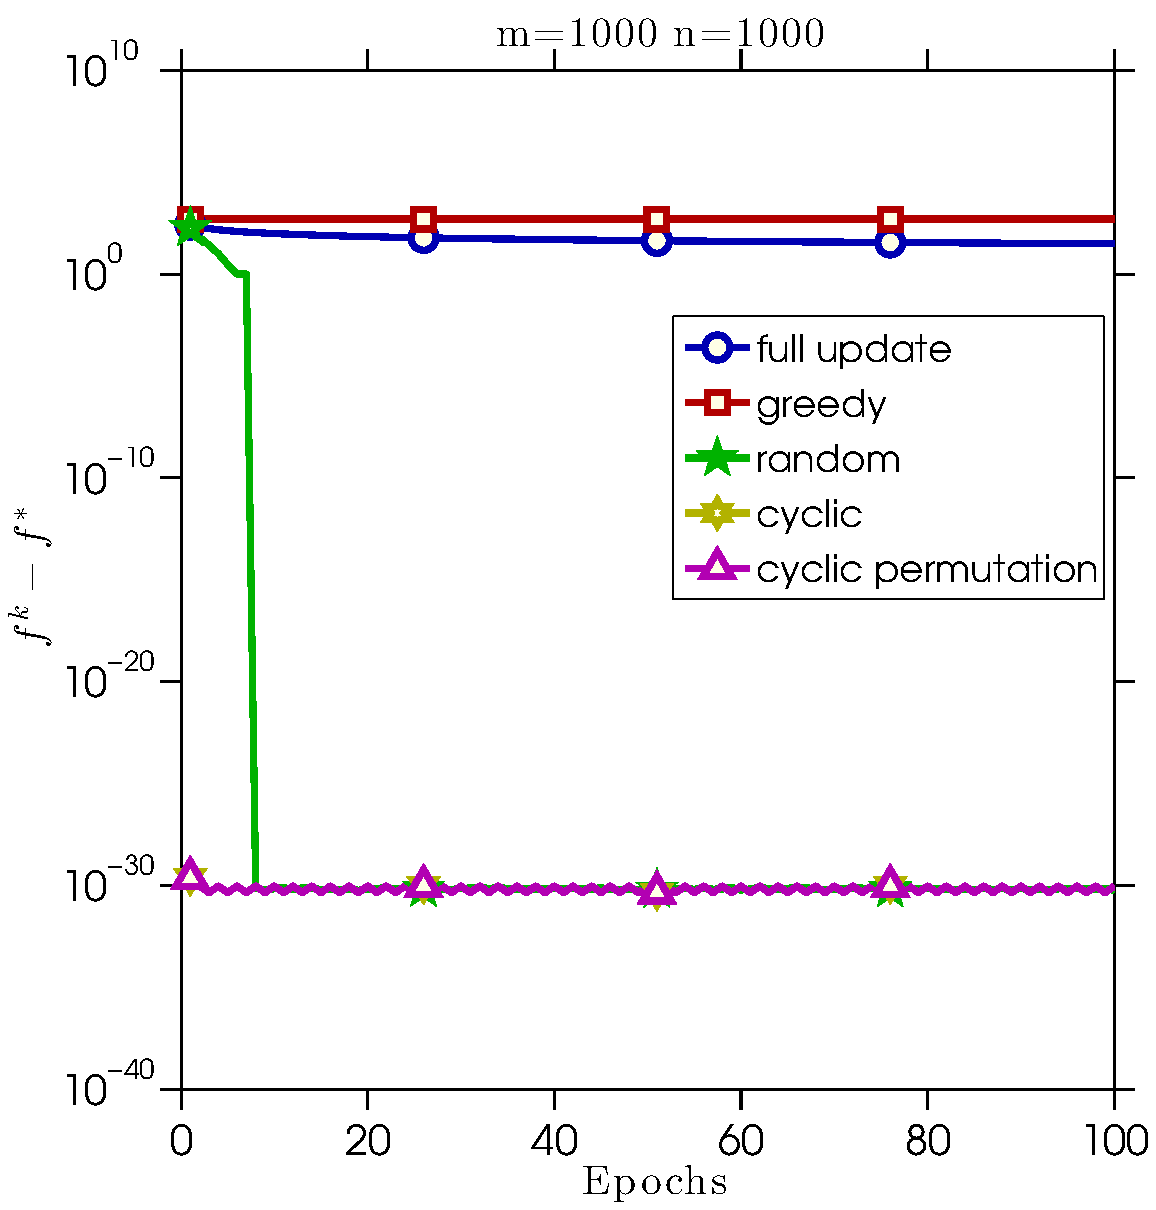
\includegraphics[width=40mm]{./figs/diag_cropped.pdf}
        \caption{Dataset I}
        \label{fig:ls_a}
    \end{subfigure} %
    \quad
    \begin{subfigure}[b]{0.3\linewidth}
        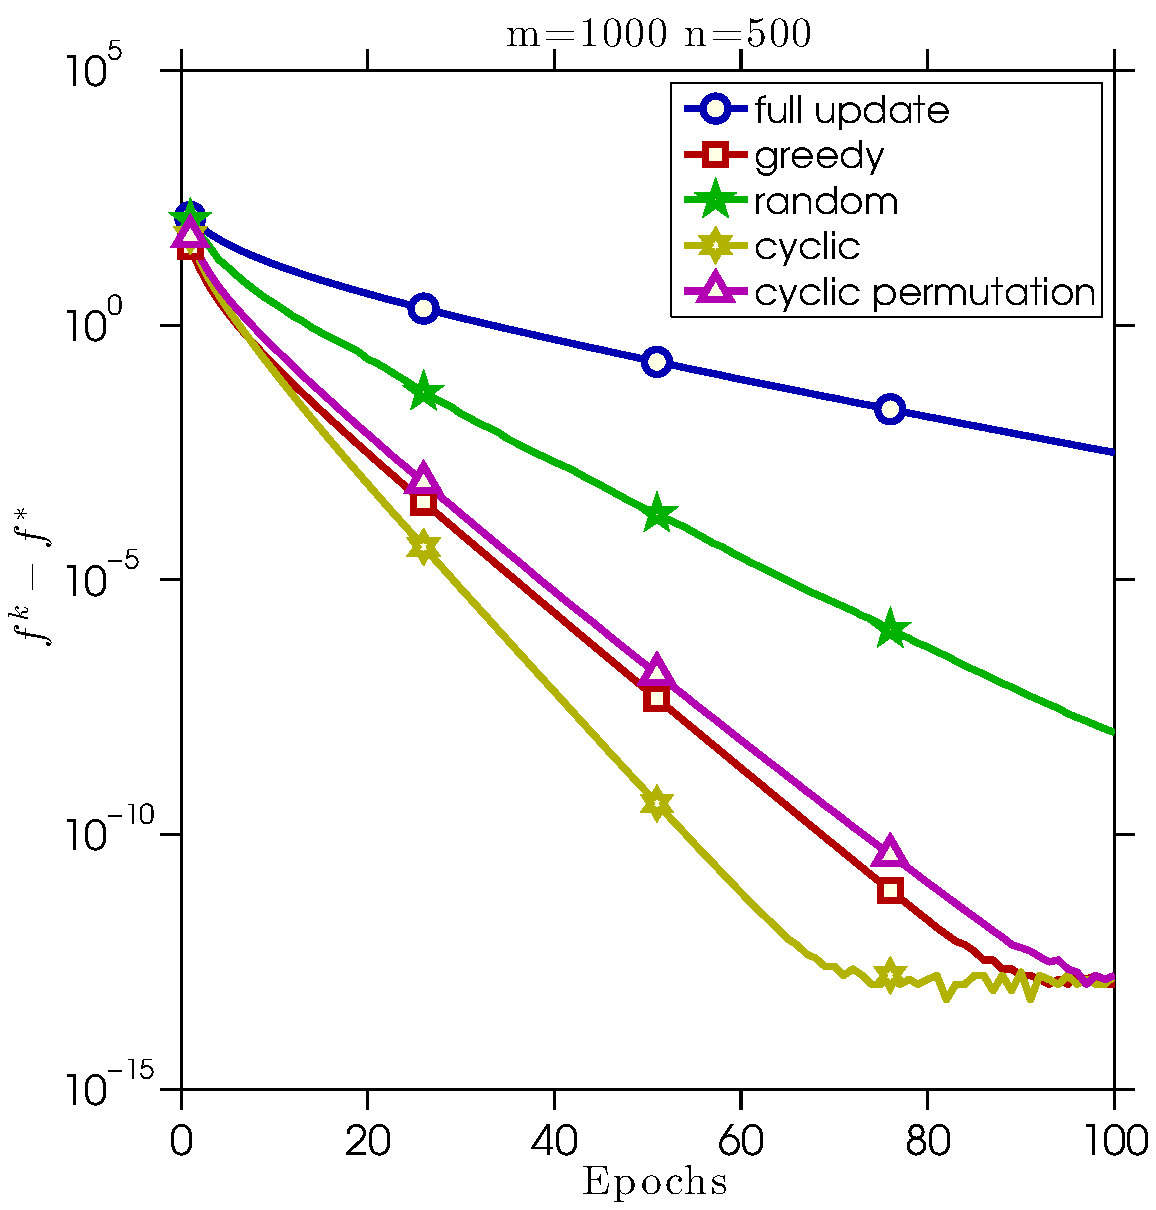
\includegraphics[width=40mm]{./figs/randn_cropped.pdf}
        \caption{Dataset II}
        \label{fig:ls_b}
    \end{subfigure} %
    \quad
    \begin{subfigure}[b]{0.3\linewidth}
        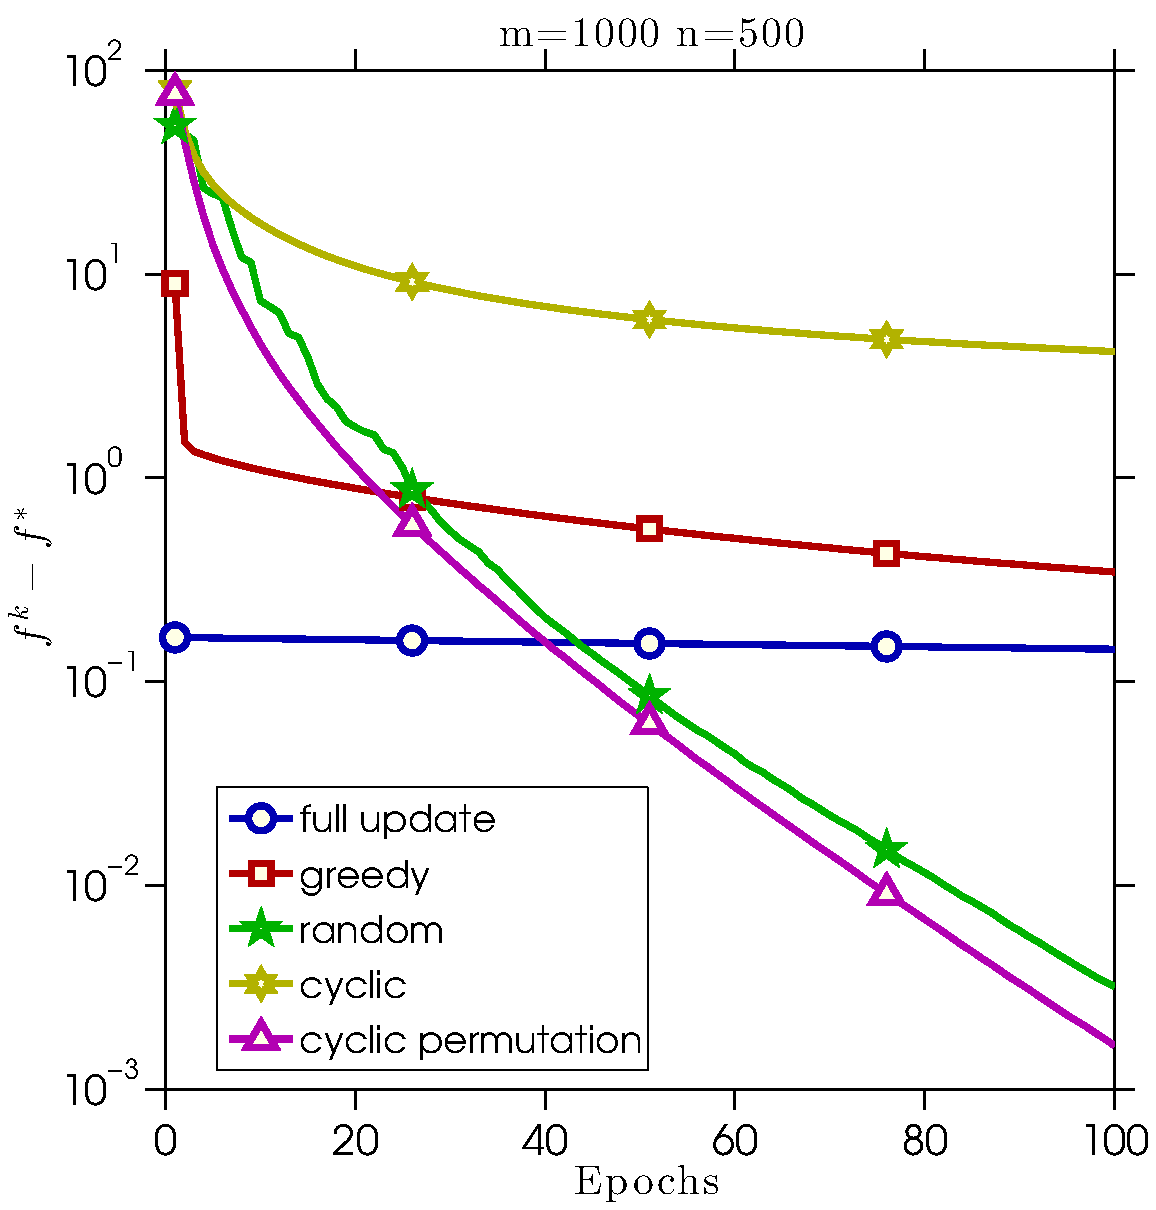
\includegraphics[width=40mm]{./figs/rand_cropped.pdf}
        \caption{Dataset III}
        \label{fig:ls_c}
    \end{subfigure} %
    \caption{Compare the convergence of four different coordinate update algorithms with full gradient descent algorithm.}
    \label{fig:3s_results}
\end{figure}
}


\subsection{Portfolio Optimization}
In this subsection, we compare the performance of the 3S splitting scheme~\eqref{eq:3op-portfolio} with the corresponding coordinate update algorithm~\eqref{eq:3op-portfolio2} for solving the portfolio optimization problem \eqref{eq:portfolio}. In this problem, our goal is to distribute our investment resources to all the assets so that the investment risk is minimized and the expected return is greater than $r$. This test uses two datasets, which are summarized in Table \ref{tab:3s-data}. The NASDAQ dataset is collected through Yahoo! Finance. We collected one year (from 10/31/2014 to 10/31/2015) of historical closing prices for 2730 stocks. 

\begin{table}[htbp]
\centering
 \begin{tabular}{rrr}
  \toprule
    & Synthetic data  & NASDAQ data\\
   \midrule
   Num. assets (N) & 1000 & 2730 \\
   Expected return rate & 0.02 & 0.02 \\
   Asset return rate & \texttt{3 * rand(N, 1) - 1} & mean of 30 days return rate \\
   Risk & covariance matrix + $0.01\cdot I$ & positive definite matrix \\
   \bottomrule
\end{tabular}
 \caption{Two datasets for portfolio optimization \label{tab:3s-data}}
\end{table}

In our numerical experiments, for comparison purposes, we first obtain a high accurate solution by solving \eqref{eq:portfolio} with an interior point solver. For both full update and coordinate update, $\eta_k$ is set to 0.8. However, we use different $\gamma$. For 3S full update, we used the step size parameter $\gamma_1 = \frac{2}{\|Q\|_2}$, and for 3S coordinate update, $\gamma_2 = \frac{2}{\max\{Q_{11}, ..., Q_{NN}\}}$. In general, coordinate update can benefit from more relaxed parameters. The results are reported in Figure \ref{fig:3s_results}. We can observe that the coordinate update method converges much faster than the 3S method for the synthetic data. This is due to the fact that $\gamma_2$ is much larger than $\gamma_1$. However, for the NASDAQ dataset, $\gamma_1 \approx \gamma_2$, so 3S coordinate update is only moderately faster than 3S full update.

\begin{figure} \centering
    \begin{subfigure}[b]{0.45\linewidth}
        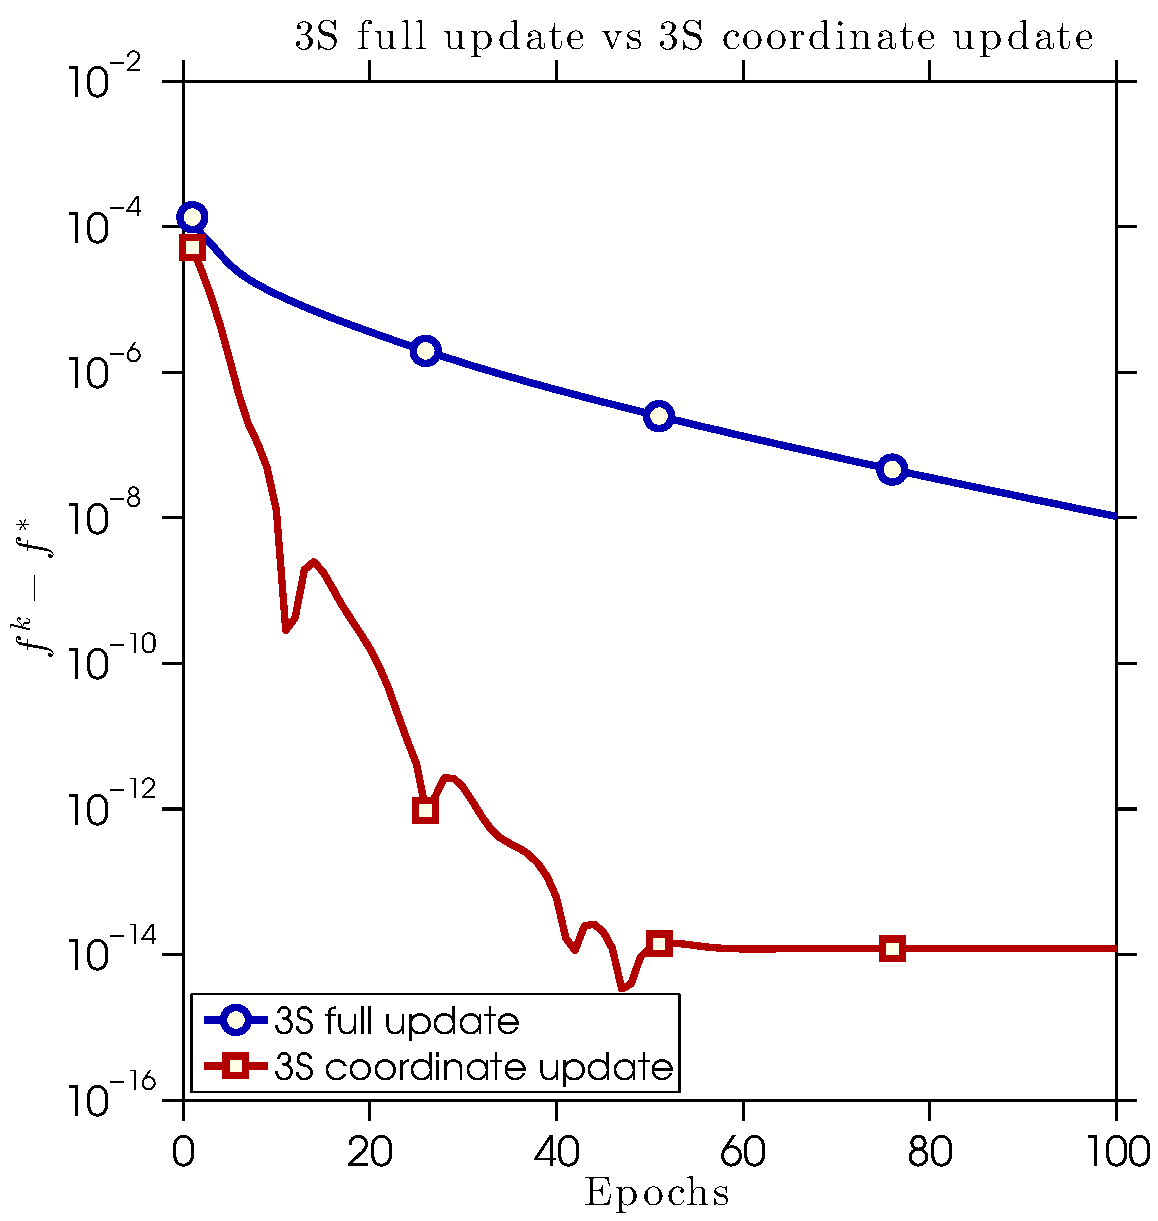
\includegraphics[width=60mm]{./figs/synth_data_f_err_cropped}
        \caption{Synthesis dataset}
        \label{fig:3s_synth}
    \end{subfigure} %
    \quad
    \begin{subfigure}[b]{0.45\linewidth}
        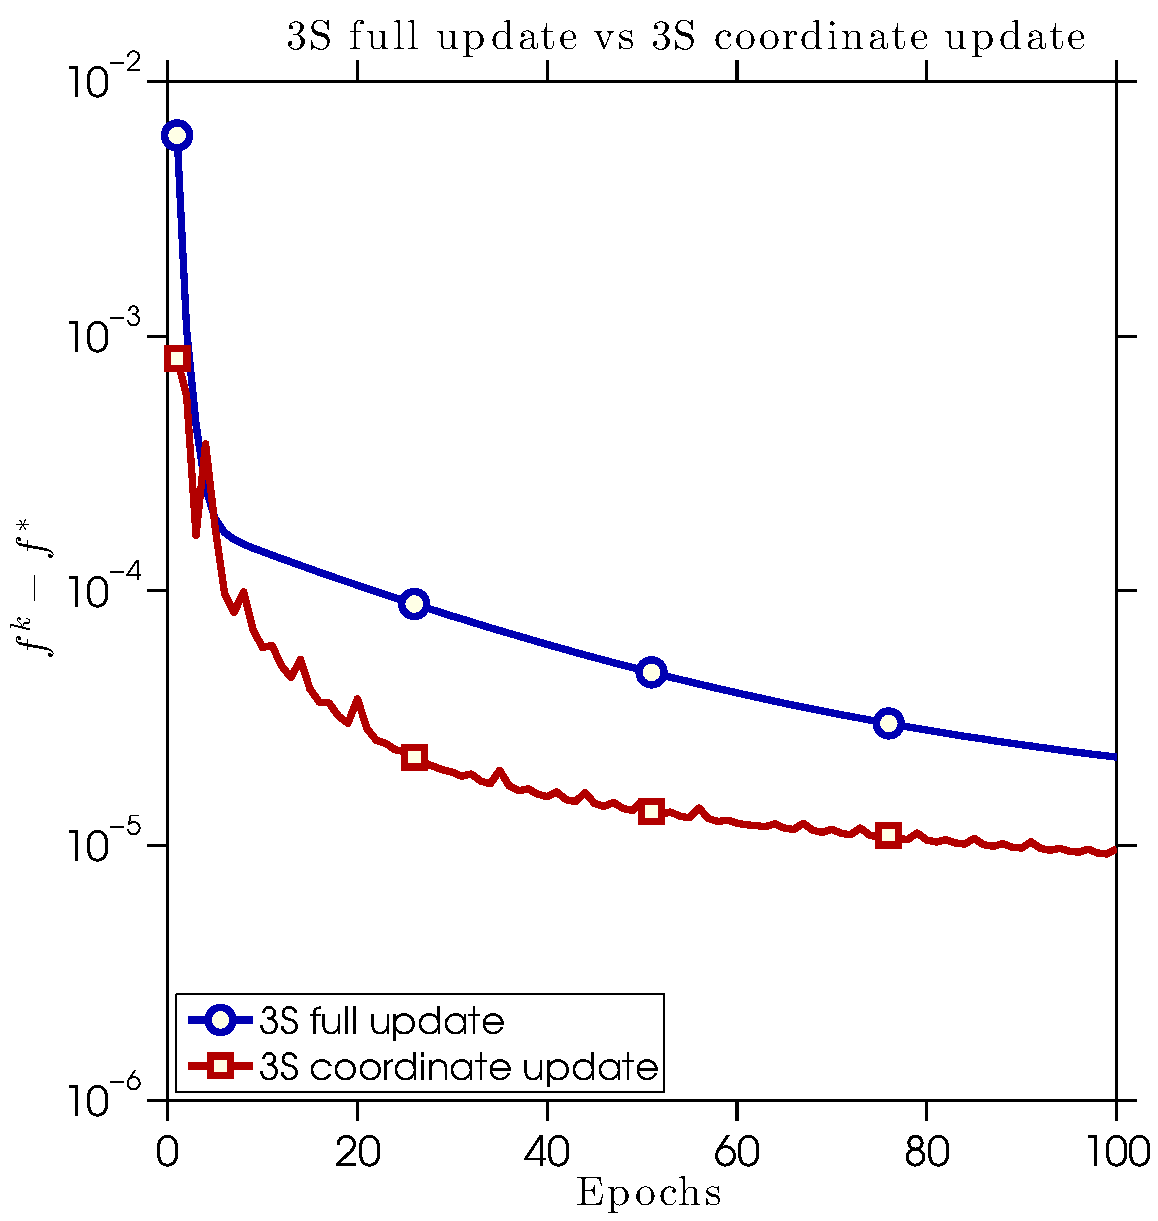
\includegraphics[width=60mm]{./figs/real_data_f_err_cropped}
        \caption{NASDAQ dataset}
        \label{fig:3s_real}
    \end{subfigure} %
    \caption{Compare the convergence of 3S full update with 3S coordinate update algorithms.}
    \label{fig:3s_results}
\end{figure}

\subsection{Computed Tomography Image Reconstruction}\label{sec:tv}
We compare the performance of algorithm~\eqref{eqn:pd_tvl2} and its corresponding coordinate version on Computed Tomography (CT) image reconstruction. We choose the standard Shepp-Logan phantom of size $256\times 256$ as the input image and apply the Siddon's algorithm~\cite{Siddon} to form the sinogram data. There are 90 parallel beam projections and, for each projection, there are 362 measurements. Then the sinogram data is corrupted with Gaussian noise. We formulate the image reconstruction problem in the form of~\eqref{eqn:tvl2}. The primal-dual full update corresponds to \eqref{eqn:pd_tvl2}. For coordinate update, the block size for $x$ is set to 256, which corresponds to a column of the image. The dual variables $s, t$ are also partitioned into 256 blocks accordingly. A block of $x$ and the corresponding blocks of $s$ and $t$ are bundled together as a single block. In each iteration, a bundled block is randomly chosen and updated. The reconstruction results are shown in Figure~\ref{fig:pds_results}. After 100 epochs, the image recovered by the coordinate version is better than that by~\eqref{eqn:pd_tvl2}. As shown in Figure~\ref{fig:pds_d}, the coordinate version converges faster than~\eqref{eqn:pd_tvl2}.

%For the numerical experiments, we choose the two dimensional Shepp-Logan phantom of dimension $256 \times 256$. The sampling matrix is obtained by ???(Ming, can you comment on this?). The sonogram data is corrupted with Gaussian noise. We present the results using 90 views. The reconstructions results are shown in Figure \ref{fig:pds_results}. We can see that within 100 epochs, the reconstructed image by PDS coordinate update method is better than the one by PDS. Figure \ref{fig:pds_d} also shows that PDS coordinate update method converges faster than PDS. 

\begin{figure}[!htb] \centering
    \begin{subfigure}{0.45\linewidth}
    	\centering
        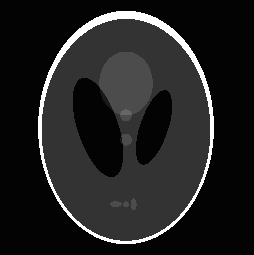
\includegraphics[width=0.9\linewidth]{./figs/phantom_img}
         \caption{Phantom image}\label{fig:pds_a}		
    \end{subfigure} %
    \quad
    \begin{subfigure}{0.45\linewidth}
    	\centering
        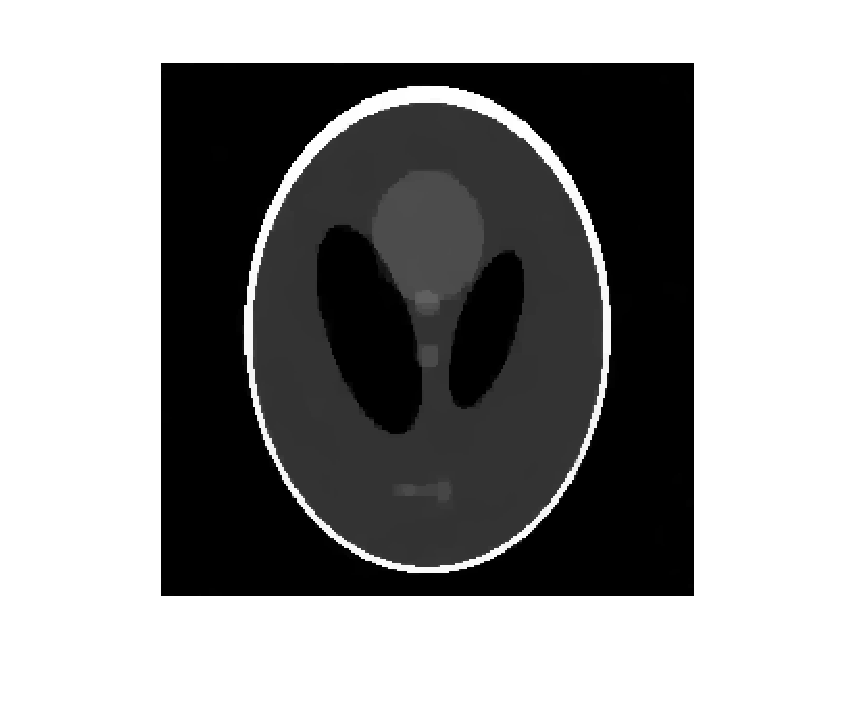
\includegraphics[width=0.9\linewidth]{./figs/phantom_pds_img}
         \caption{Recovered by PDS}\label{fig:pds_b}		        
    \end{subfigure} %
    \begin{subfigure}{0.45\linewidth}
    	\centering
        
\includegraphics[width=0.9\linewidth]{./figs/phantom_pds_coord_img}
         \caption{Recovered by PDS coord}\label{fig:pds_c}		        
    \end{subfigure} %
    \quad
    \begin{subfigure}{0.45\linewidth}
    	\centering
        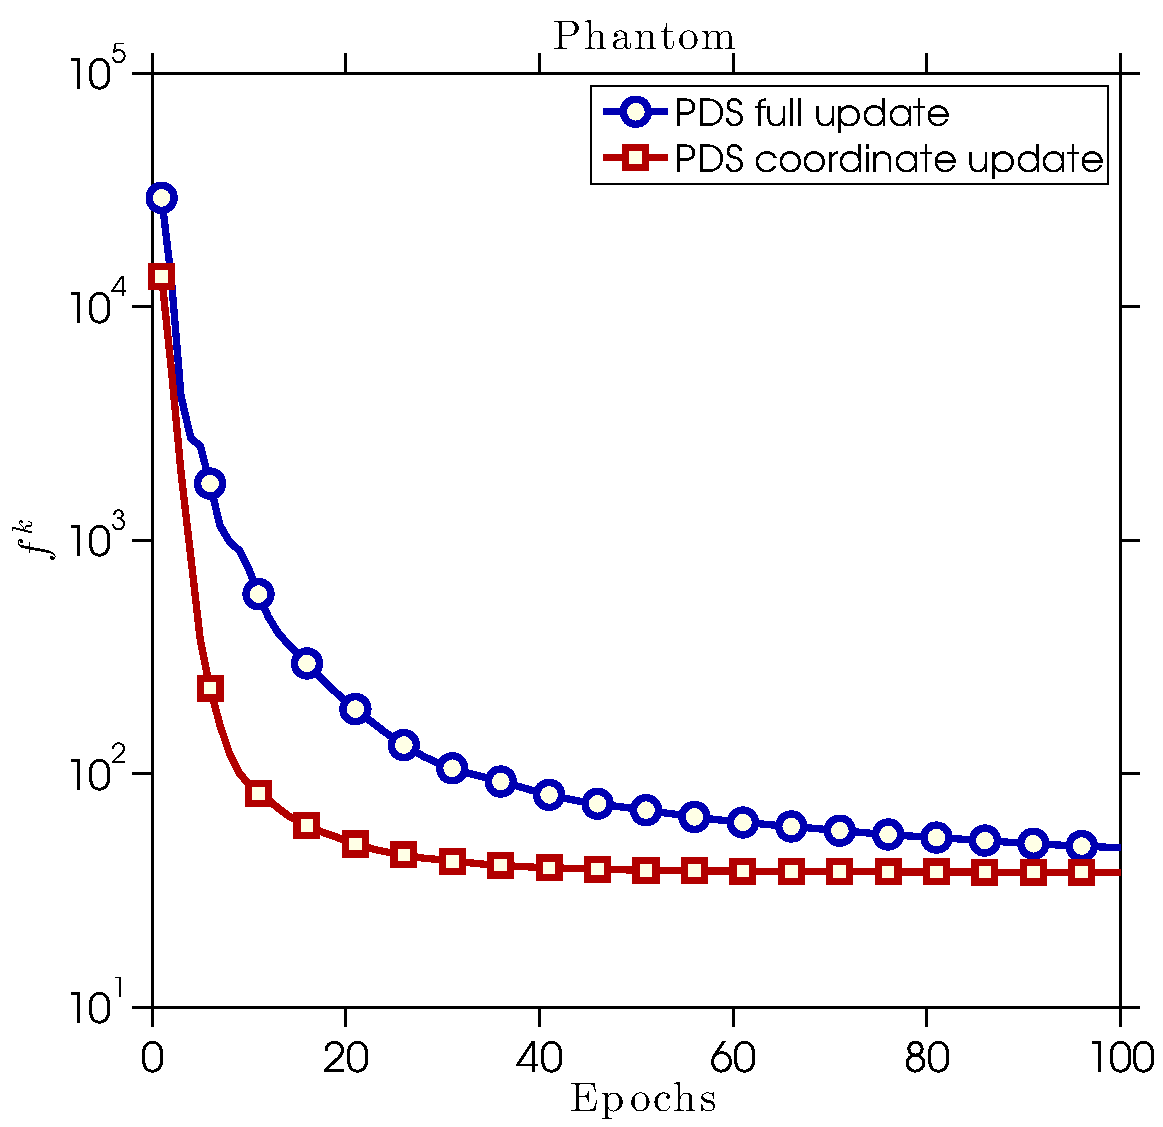
\includegraphics[width=\linewidth]{./figs/phantom_func_val_cropped}
         \caption{Objective function value}\label{fig:pds_d}		                
    \end{subfigure} %    
    \caption{CT image reconstruction.}
    \label{fig:pds_results}
\end{figure}


\subsection{$\ell_1$ Regularized Logistic Regression}
In this subsection, we compare the performance of sync-parallel coordinate update and the async-parallel coordinate update for solving the sparse logistic regression problem 
\begin{equation}\label{eqn:log}
\Min_{x \in \mathbb{R}^n} \lambda \|x\|_1 + \frac{1}{N} \sum_{i=1}^N \log\big(1 + \exp(-b_i \cdot a_i^{\top} x)\big),
\end{equation}
where $\{(a_i, b_i)\}_{i=1}^N$ is the set of sample-label pairs with $b_i \in \{1, -1\}$, $\lambda=0.0001$, and $n$ and $N$ represent the numbers of features and samples, respectively. This test uses the datasets\footnote{\url{http://www.csie.ntu.edu.tw/~cjlin/libsvmtools/datasets/}}: real-sim and news20, which are summarized in Table \ref{tab:log_data}.

\begin{table}[htbp]
\centering
 \caption{\label{tab:log_data}Two  datasets for  sparse logistic regression }
 \begin{tabular}{rrr}
\hline
  Name & \# samples & \# features \\
  \hline
 real-sim & 72, 309 & 20, 958 \\
  news20 & 19,996 & 1,355,191\\
  \hline
 \end{tabular}
\end{table}

We let each coordinate hold roughly 50 features. {Since the total number of features is not divisible by 50, some coordinates have 51 features.} We let each thread draw a coordinate uniformly at random at each iteration. We stop all the tests after 10 epochs since they have nearly identical progress per epoch. %The size of the block of coordinates is set to 50. In each iteration, each core randomly draws a block and updates it.
The step size is set to $\eta_k=0.9,\,\forall k$. Let $A = [a_1, \ldots, a_N]^{\top}$ and $b = [b_1, ..., b_N]^{\top}$. In global memory, we store $A, b$ and $x$. We also store the product $Ax$ in global memory so that the forward step can be efficiently computed. Whenever a coordinate of $x$ gets updated, $Ax$ is immediately updated at a low cost. Note that if $Ax$ is \emph{not} stored in global memory, every coordinate update will have to compute $Ax$ from scratch, which involves the entire $x$ and will be very expensive.  %Note that the renewal of $Ax$ can be computed  efficiently, and it enables ARock to have the same per epoch computational complexity as that of the sequential FBS.

Table \ref{tab:log_time} gives the running times of  the sync-parallel and async-parallel implementations on the two datasets. We can observe that async-parallel achieves almost-linear speedup, but sync-parallel scales very poorly as we explain below.

In the sync-parallel implementation,  all the running cores have to wait for the last core to finish an iteration, and therefore if a core has a large load, it slows down the iteration. Although every core is (randomly) assigned to roughly the same number of features (either 50 or 51 components of $x$) at each iteration, their  $a_i$'s have very different numbers of nonzeros, and the core with the largest number of nonzeros is the slowest. (Sparse matrix computation is used for both datasets, which are very large.) As more cores are used,  despite that they altogether do more work at each iteration,  the per-iteration time reduces as the slowest core tends to be slower. On the other hand, async-parallel coordinate update does not suffer from the  load imbalance. Its performance grows nearly linear with the number of cores.

Finally, we have observed that the progress toward solving \eqref{eqn:log} is mainly a function of the number of epochs and does not change appreciably  when the number of cores increases or between sync-parallel and async-parallel. Therefore, we always stop at 10 epochs.


\begin{table}[htbp]
\centering
 \begin{tabular}{|c|r|r|r|r|r|r|r|r|}
  \hline
  \multirow{3}{*}{\# cores} & \multicolumn{4}{|c|}{real-sim} & \multicolumn{4}{c|}{news20} \\
  \cline{2-9}
  & \multicolumn{2}{|c|}{time (s)} &  \multicolumn{2}{c|}{speedup} &  \multicolumn{2}{c|}{time (s)} & \multicolumn{2}{c|}{speedup}\\
  \cline{2-9}
  & async & sync &  async & sync &  async & sync &  async & sync \\
  \hline
   1 &   81.6 &  82.1 & 1.0   & 1.0 & 591.1   & 591.3 & 1.0   & 1.0\\
   2 &   45.9   &  80.6 & 1.8   & 1.0 & 304.2   & 590.1 & 1.9   & 1.0\\
   4 &   21.6   &  63.0   & 3.8   & 1.3 & 150.4   & 557.0 & 3.9   & 1.1\\
   8 &   16.1   &  61.4   & 5.1   & 1.3 & 78.3     & 525.1 & 7.5   & 1.1\\
   16 & 7.1     &  46.4   & 11.5 & 1.8 & 41.6     & 493.2 & 14.2 & 1.2\\
  \hline
 \end{tabular}
 \caption{\label{tab:log_time}Running times of async-parallel and sync-parallel FBS implementations for $\ell_1$ regularized logistic regression on two datasets. Sync-parallel has very poor speedup  due to the large distribution of coordinate sparsity and thus the large load imbalance across cores.}
\end{table}
